При наблюдении голографических изображений, полученных по схеме Габора,
действительное и мнимое изображения создают взаимные помехи: изображения 
$S'$ и $S''$ находятся на одной прямой с точкой, в которой расположен глаз наблюдателя (рис. \ref{img::3_50}).
Помехи создаются также возникающей при восстановлении плоской волной, бегущей
вдоль оси $z$ и не несущей информации об объекте. В 1962 году Лейт и Упатниекс предложили использовать для записи голограммы наклонный опорный пучок.

\begin{wrapfigure}{l}{0.3\linewidth}
  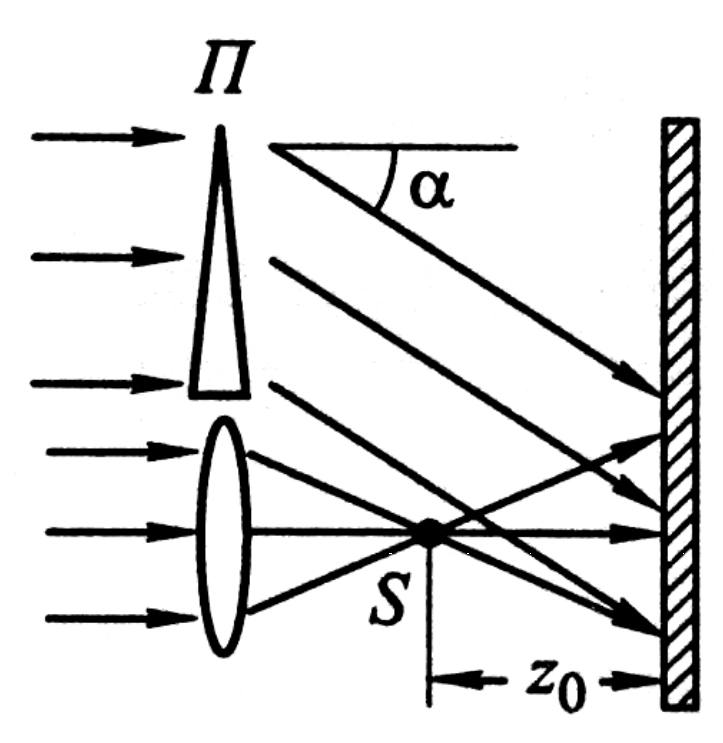
\includegraphics[width=\linewidth]{3.53.png}
  \caption{Наклонный опорный пучок}
  \label{img::3_53}
\end{wrapfigure}

Проследим, каким образом введение опорного наклонного пучка обеспечивает 
возможность независимого (без взаимных помех) наблюдения действительного
и мнимого изображений. На рис. \ref{img::3_53} \quot{предметом} является 
\quot{точечный источник} $S$. Наклон опорного пучка обеспечивается призмой
$\Pi$. Поле предметной волны на голограмме есть
$$
f_{\Pi}(x, y) = a \e^{\iu \frac{k}{2z_0}\left(x^2+y^2\right)}
$$

(мы вновь используем параболическое приближение). Наклонная опорная волна 
имеет вид $f_0 = a\e^{\iu u_0x}$, где $u_0 = k \sin{\alpha}$ ~---~ 
пространственная частота опорной волны. Мы полагаем, что волны
имеют равные амплитуды и создают в начале координат плоскости $xy$
(плоскость голограммы) синфазные колебания. Функция пропускания
проявленной голограммы, пропорциональная интенсивности суммарной волны при 
записи, имеет вид
$$
t(x, y) \sim 
\left|
a\e^{\iu u_0 x} + a \e^{\iu \frac{k}{2z_0}\left(x^2+y^2\right)}
\right|^2 .
$$

Слагаемые, ответственные за появление действительного и мнимого изображения 
при восстановлении, можно записать в виде:
\begin{align*}
f_3(x, y) \sim
b \e^{\iu \frac{k}{2z_0}
\left(
  \left(
    x + z_0 \sin{\alpha}
  \right)^2
  +y^2
\right)
}, &&
f_4(x, y) \sim
b \e^{ -\iu \frac{k}{2z_0}
  \left(
  \left(
  x + z_0 \sin{\alpha}
  \right)^2
  +y^2
  \right)
},
\end{align*}

\begin{wrapfigure}{l}{0.4\linewidth}
  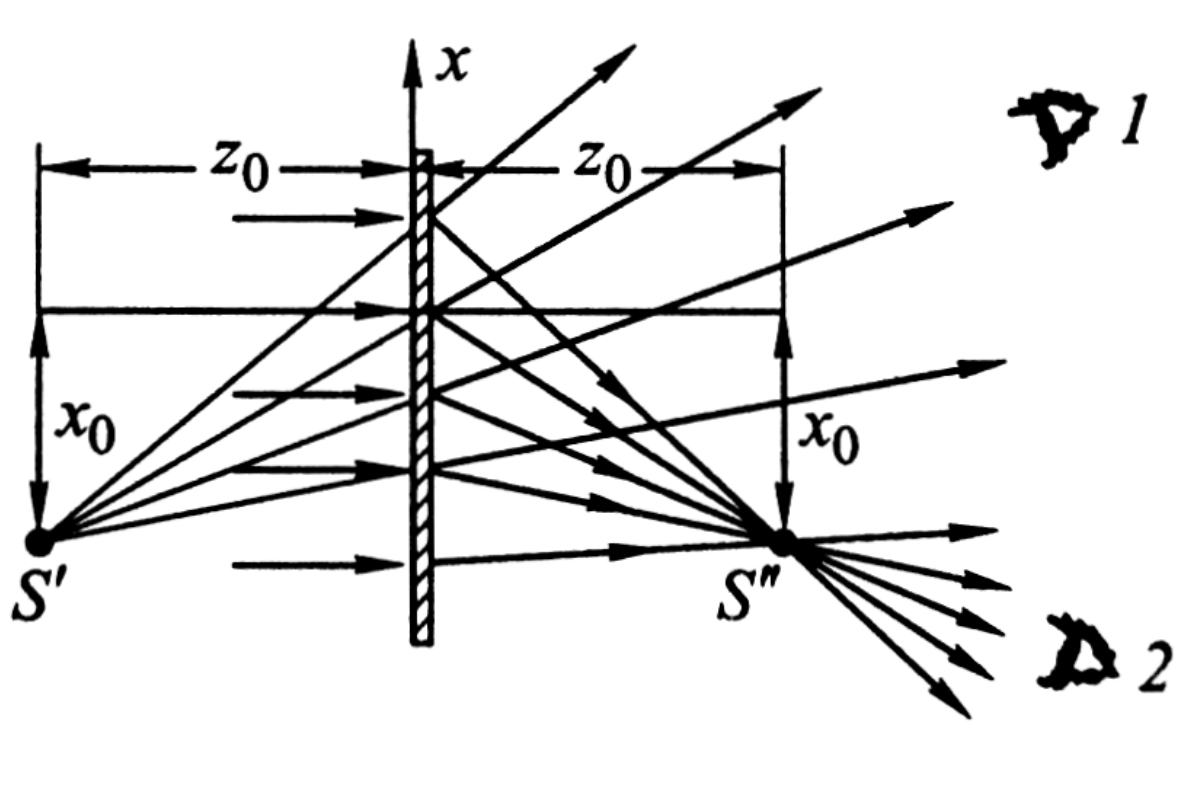
\includegraphics[width=\linewidth]{3.54.png}
  \caption{Мнимые и действительные изображения в схеме с наклонным пучком}
  \label{img::3_54}
\end{wrapfigure}

где $b$ ~---~ комплексная константа. Выражение $f_3(x,y)$ представляет собой
поле, которое создавал бы в плоскости $z = 0$ точечный источник, находящийся в точке с координатами
$x_0 = -z_0 \sin{\alpha}$, $y = 0$, на расстоянии $z_0$ слева от голограммы.
Это мнимое изображение предмета $S'$ (рис. \ref{img::3_54}).
Соответственно $f_4(x,y)$ описывает поле сходящейся в точку $S''$
сферической волны. Эта точка находится справа от голограммы на расстоянии
$z_0$ и смещена относительно оси $z$ на расстояние $x_0 = -z_0 \sin{\alpha}$.
Это ~---~ действительное изображение. Мы видим, что введение наклонного
опорного пучка приводит к сдвигу мнимого и действительного изображений таким образом, что наблюдатель может рассматривать их из
разных положений (1 и 2 на рис. \ref{img::3_54}), в которых они не создают взаимных помех.
Разумеется, угол наклона опорного пучка $\alpha$ (т.е. его пространственная частота) должен быть выбран правильно: чем шире
пространственный спектр предметной волны, тем больше должен быть угол наклона опорного пучка, 
при котором волны, ответственные за создание действительного и мнимого изображений, не создают взаимных помех.